We organize our results into two subsections, with each subsection focusing on results from a phase of experiments.
%\vspace{-2mm}
\subsection{Phase-I Results Using Cloverleaf3D Simulation Code}
\label{sec:experiment1}
We report the results of \textbf{Phase-I} experiments that include a weak scaling study, \textbf{C-I}, and \textbf{C-II}.
%\vspace{-2mm}
\subsubsection{Weak Scaling Study} 
We considered 17 configurations of the Cloverleaf3D simulation in our weak scaling \textbf{Phase-I} study. 
%
Our experiment configurations span $81^{3}$ cells across 2 MPI ranks on 1 CN to $812^{3}$ cells across 2048 MPI ranks on 512 CNs, with each MPI rank operating on an approximately $64^{3}$ grid.
%
In each case, one GPU was assigned to every MPI rank, and we varied the number of ranks per CN.
%
With respect to the number of MPI ranks on each CN, we ran 1 test using 2 ranks, 10 tests using 4 ranks, and 6 tests using 6 ranks.
%
For each run, we terminated the simulation after 500 cycles.
%
Given the variation in grid size, each test reached a different stage of the simulation.
%
As the simulation grid size increased, the step size used by the simulation decreased.
%
%We believe this was an acceptable assumption for most simulation codes.
%
With respect to parameterization of the Lagrangian flow map computation, we used a storage interval of 25 cycles and a data reduction of 1:8 ($\approx32,768$ particles seeded per MPI rank) for every test.

\textbf{Execution Time.} Figure~\ref{fig:total_time} compares the average total time required per step by Lagrangian$_{Dist}$ and Lagrangian$_{Local}$.
%
As the scale of the simulation increased, the cost of communication dominated the execution time for Lagrangian$_{Dist}$.  
%
In comparison, Lagrangian$_{Local}$ scaled better because each MPI rank operated independently.
%
For the range of configurations considered, Lagrangian$_{Local}$ demonstrated up to 4x speed-up over Lagrangian$_{Dist}$.
%
Further, we expect this speed-up would increase even more as the scale of the simulation increases.
%
The cost of particle advection (for both techniques) increased as the scale of the simulation increased.
%
However, this increase in particle advection cost was attributed to the difference in each test domain and the RK4 kernel that performed velocity field interpolation.
%
%We believe the performance of the kernel considering the parameters of cell size, step size, and vector field is worth future investigation.
%
Further, use of a faster particle advection kernel would result in greater speed-ups for Lagrangian$_{Local}$.
\begin{figure}[!b]
\centering
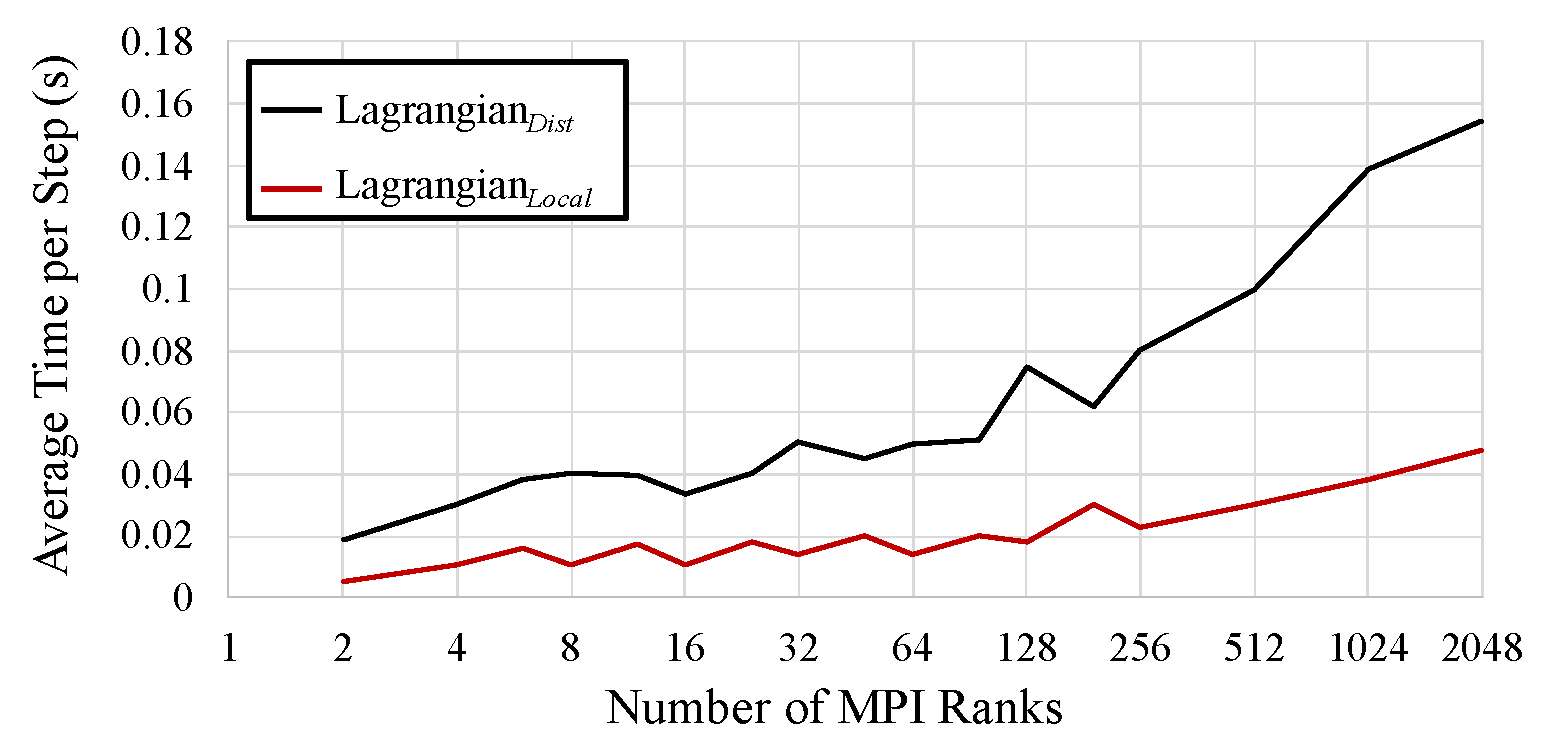
\includegraphics[width=0.9\linewidth]{Images/total_time.pdf}
\caption{Weak scaling study using in situ infrastructure to compute Lagrangian flow maps for the Cloverleaf3D data set.}
\label{fig:total_time}
\end{figure}

\begin{figure}[!b]
\vspace{-4mm}
\begin{subfigure}{0.495\linewidth}
\centering
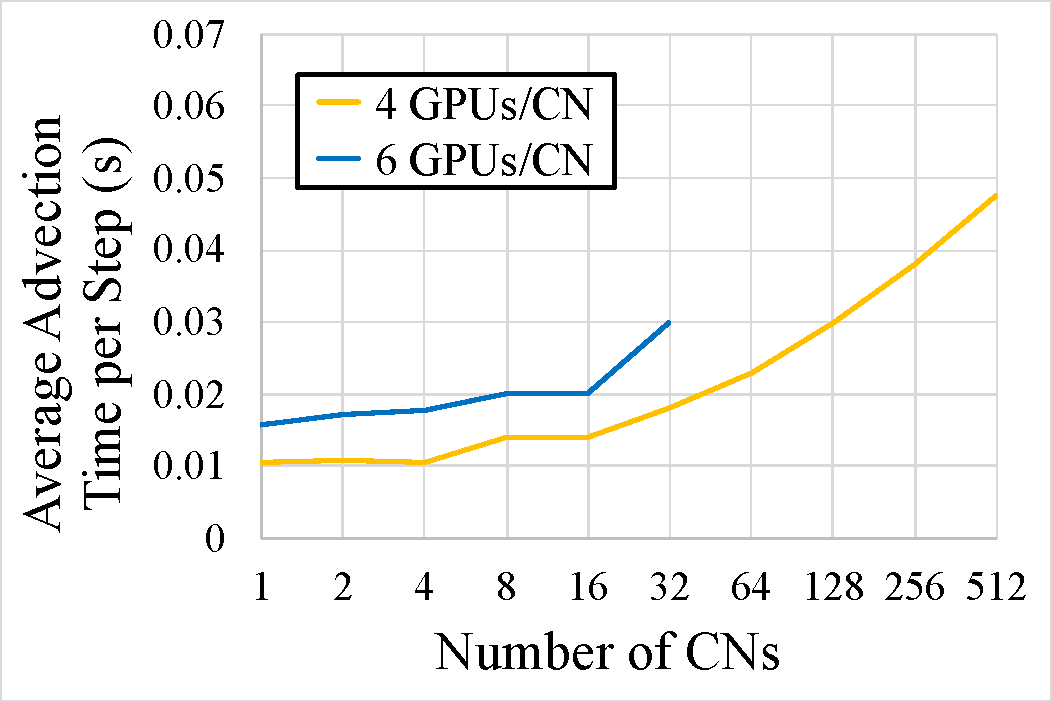
\includegraphics[width=\linewidth]{Images/advection_time2.pdf}
\vspace{-3mm}
\caption{Costs of particle advection.}
\label{fig:advection}
\end{subfigure}
\begin{subfigure}{0.495\linewidth}
\centering
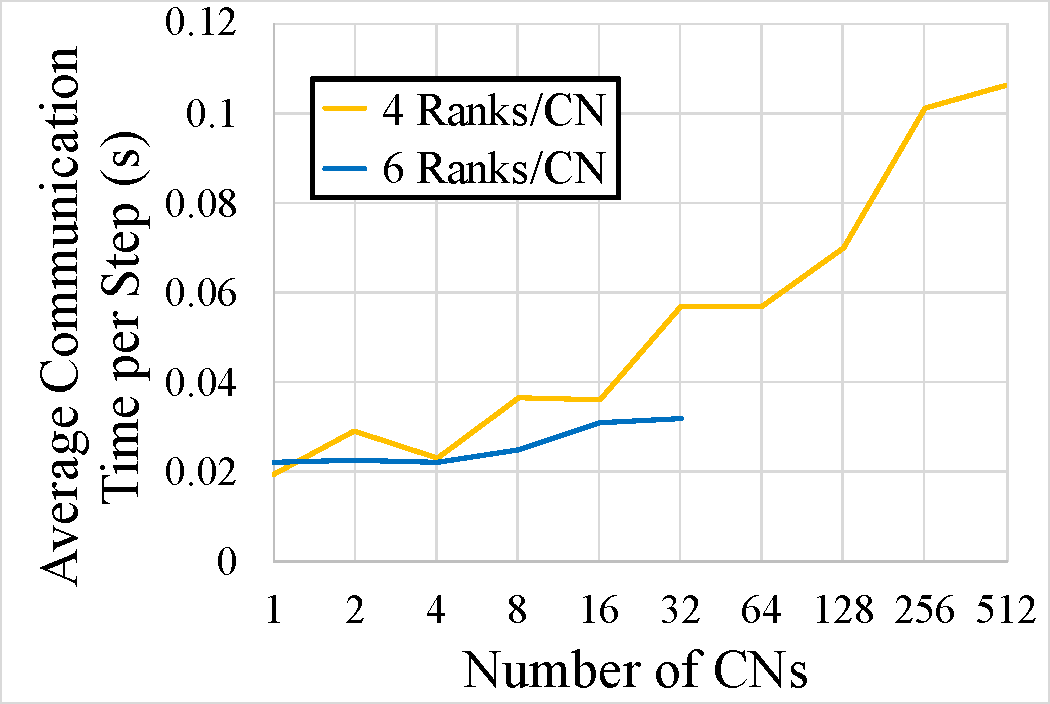
\includegraphics[width=\linewidth]{Images/communication_time2.pdf}
\vspace{-3mm}
\caption{Costs of communication.}
\label{fig:communication}
\end{subfigure}
\caption{\fix{Results for weak scaling the number of GPUs or ranks (4 or 6) per compute node. Lagrangian$_{Local}$ particle advection costs are plotted in~\ref{fig:advection} and Lagrangian$_{Dist}$ communication costs are in~\ref{fig:communication}. While particle advection performed better with fewer GPUs sharing memory on a single compute node~(\ref{fig:advection}), communication benefitted from MPI optimizations when more ranks execute on a single compute node~(\ref{fig:communication}).}} 
\label{fig:gpu_nodes}
\end{figure}


%\textbf{Varying GPUs/Ranks per Compute Node.}
%Since each CN on Summit has 6 GPUs, a simulation can be configured in several ways.
%
%In our tests, each rank has a dedicated GPU and operates on approximately the same number of particles.
%
The ``sawtooth'' nature of the line curves in Figure~\ref{fig:total_time} is the result of a series of test configurations alternating between 4 and 6 ranks per CN.
%
Varying the number of ranks (each using 1 GPU) on each CN impacted both particle advection and communication costs.
%
%Using data points from our weak scaling \textbf{Phase-I} study, we analyze these effects.
%
%
%Figure~\ref{fig:advection} isolates the costs of particle advection per step of Lagrangian$_{Local}$.
%
Particle advection performed better with 4 GPUs per CN versus 6.
%
Use of shared memory by multiple GPUs on a single CN and saturation of the NVLink by the VTK-m particle advection kernel caused this effect.
%
%
%Figure~\ref{fig:communication} shows the difference in communication costs per step for Lagrangian$_{Dist}$.
%
In contrast, the MPI communication cost showed a reduction when using 6 ranks versus 4 per CN. 
%
%The data points using 4 ranks per CN show poor scalability as the number of CNs continues to increase.
%
On-node MPI communication optimizations contributed to better performance when grouping a larger number of MPI ranks on each CN. 
%
However, the communication cost of inter-node remained high in comparison to intra-node.
%
Configurations using 4 ranks per CN showed particularly poor scalability as the number of CNs increased.
%
%Although these results inform computational performance, the specific configuration is determined by the simulation.
%
These weak scaling trends can be observed by isolating the individual costs. 
%
Figure~\ref{fig:advection} shows particle advection costs per step for Lagrangian$_{Local}$ and Figure~\ref{fig:communication} shows communication costs per step for Lagrangian$_{Dist}$. 

\textbf{Reconstruction Accuracy.}
We calculated the reconstruction accuracy for eight of the Lagrangian$_{Local}$ weak scaling \textbf{Phase-I} configurations, which we labeled T1 through T8~(see Figure~\ref{fig:clover_plot}). 
%
Configurations terminated 2\%-5\% of particles and consequently stored 95\%-98\% of all initially seeded trajectories. 
%
We measured the accuracy of reconstructing the discarded trajectories only and present the results using violin plots in Figure~\ref{fig:clover_plot}.
%
As the simulation grid resolution increased, the grid cell size and particle advection step size decreased, while the total number of particles sampling the domain increased. 
%
Over 75\% of discarded trajectories have reconstruction error under 25\% of a GCS from the ground truth.
%
Further, this trend was observed across all the 8 test configurations we reconstructed. 

Reconstruction accuracy, however, was not constant across all storage intervals and demonstrates temporal patterns.
%
%
Figure~\ref{fig:clover_map} uses a heatmap for reconstruction accuracy across every interval of a Cloverleaf3D test. 
%
Measuring reconstruction accuracy for individual intervals could provide insight into the suitability to compute local Lagrangian flow maps versus incur communication costs to retain all particles trajectories.
%
%This concept can extend to consider spatial patterns as well. 
%
\begin{figure}[!t]
\vspace{-2mm}
\centering
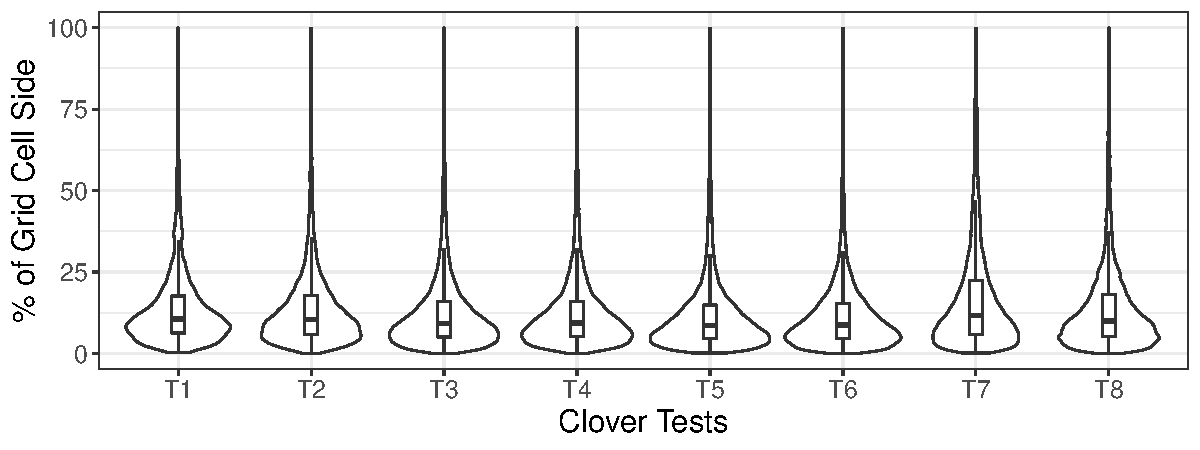
\includegraphics[width=\linewidth]{Images/Clover_Tests_1_8.pdf}
\caption{The distribution of the reconstruction error for eight Cloverleaf3D tests (labeled T1 through T8). The grid dimensions increase l-r from $81^{3}$ to $204^{3}$ over 500 cycles.}
\label{fig:clover_plot}
\vspace{-3mm}
\end{figure}

\begin{figure}[!t]
\centering
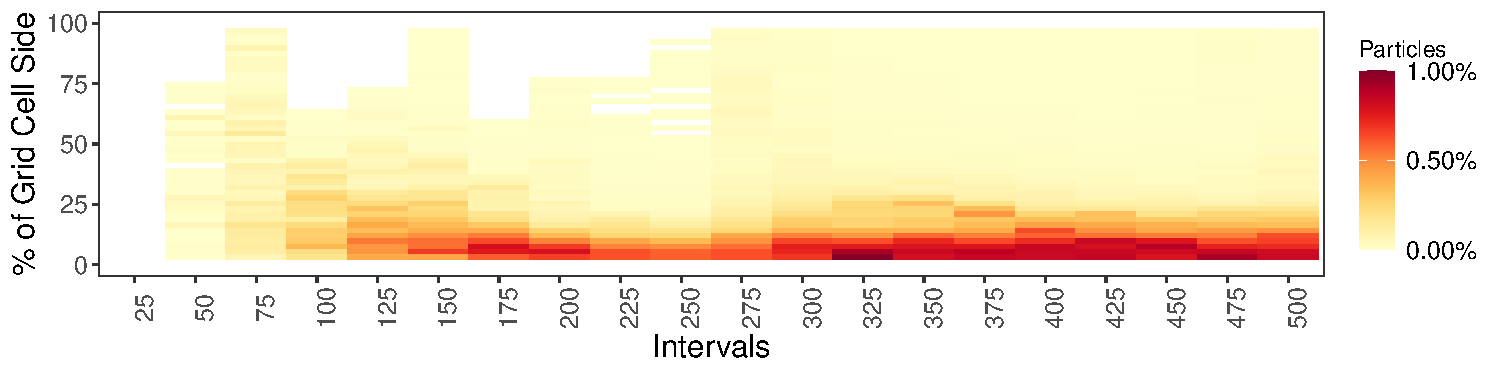
\includegraphics[width=\linewidth]{Images/Clover_Intervals_T8.pdf}
\caption{The Cloverleaf3D data set reconstruction error for all the intervals of a single test configuration~(T8).}
\vspace{-2mm}
\label{fig:clover_map}
\end{figure}

%
Overall, using Lagrangian$_{Local}$ with a storage interval of 25 cycles and 1:8 data reduction factor, the complete Lagrangian flow map was reconstructed accurately (under 100\% of GCS) while providing speed-ups of 2x-4x for the Cloverleaf3D data set.

%\vspace{-2mm}
\subsubsection{C-I Results} 
%
\begin{figure}[!t]
\centering
%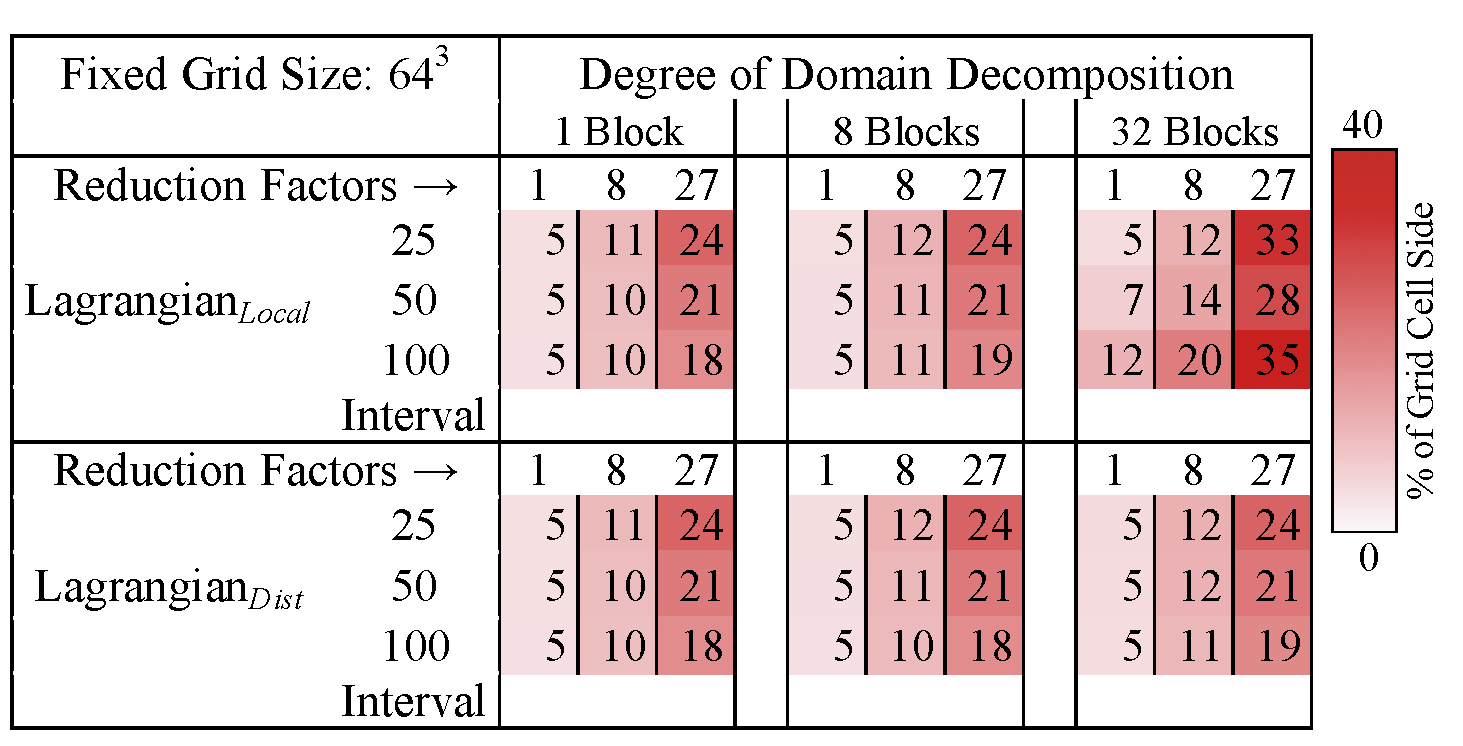
\includegraphics[width=\linewidth, trim={1.25cm 6.5cm 1.25cm 6.5cm}, clip]{Images/strongscaling.pdf}
%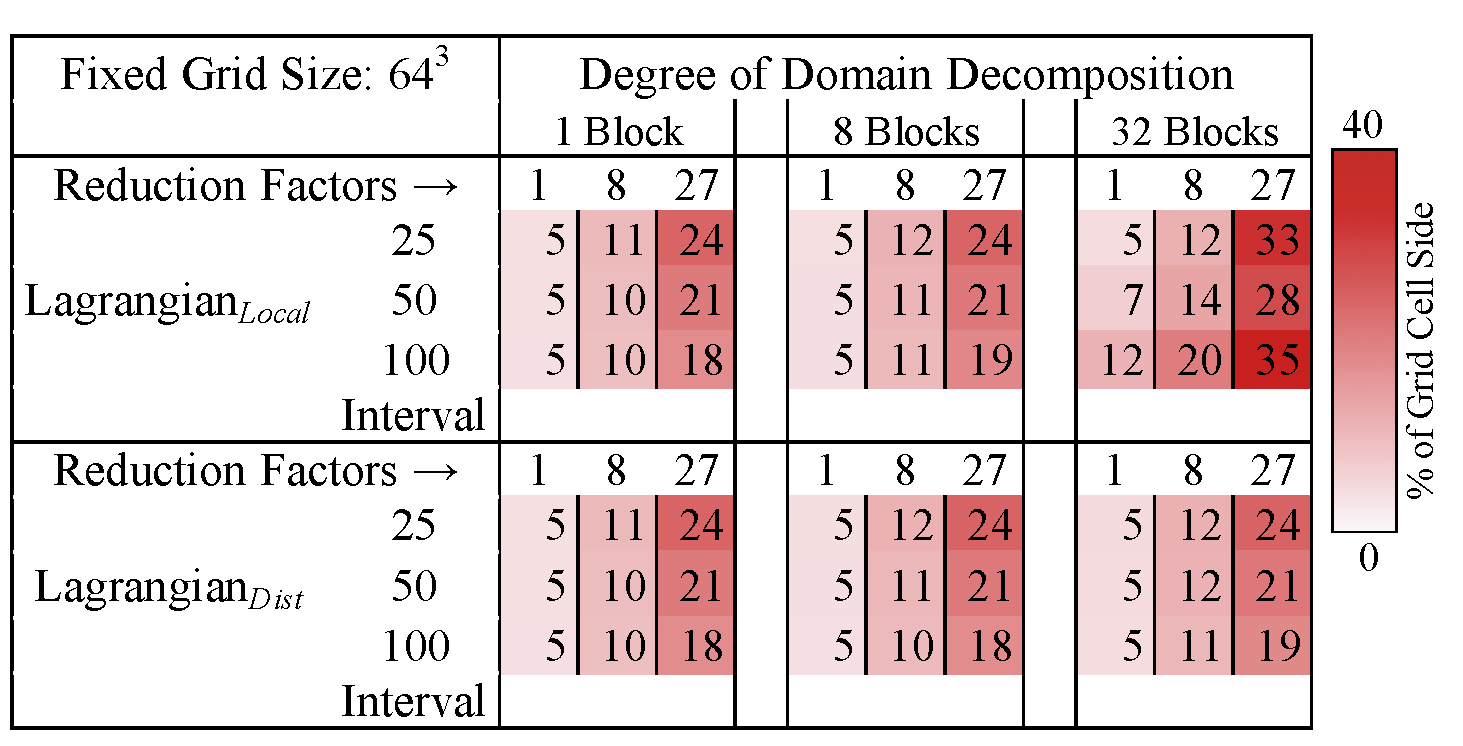
\includegraphics[width=\linewidth, trim={1.5cm, 16.8cm, 2cm, 1.8cm}, clip]{Images/strongscaling.pdf}
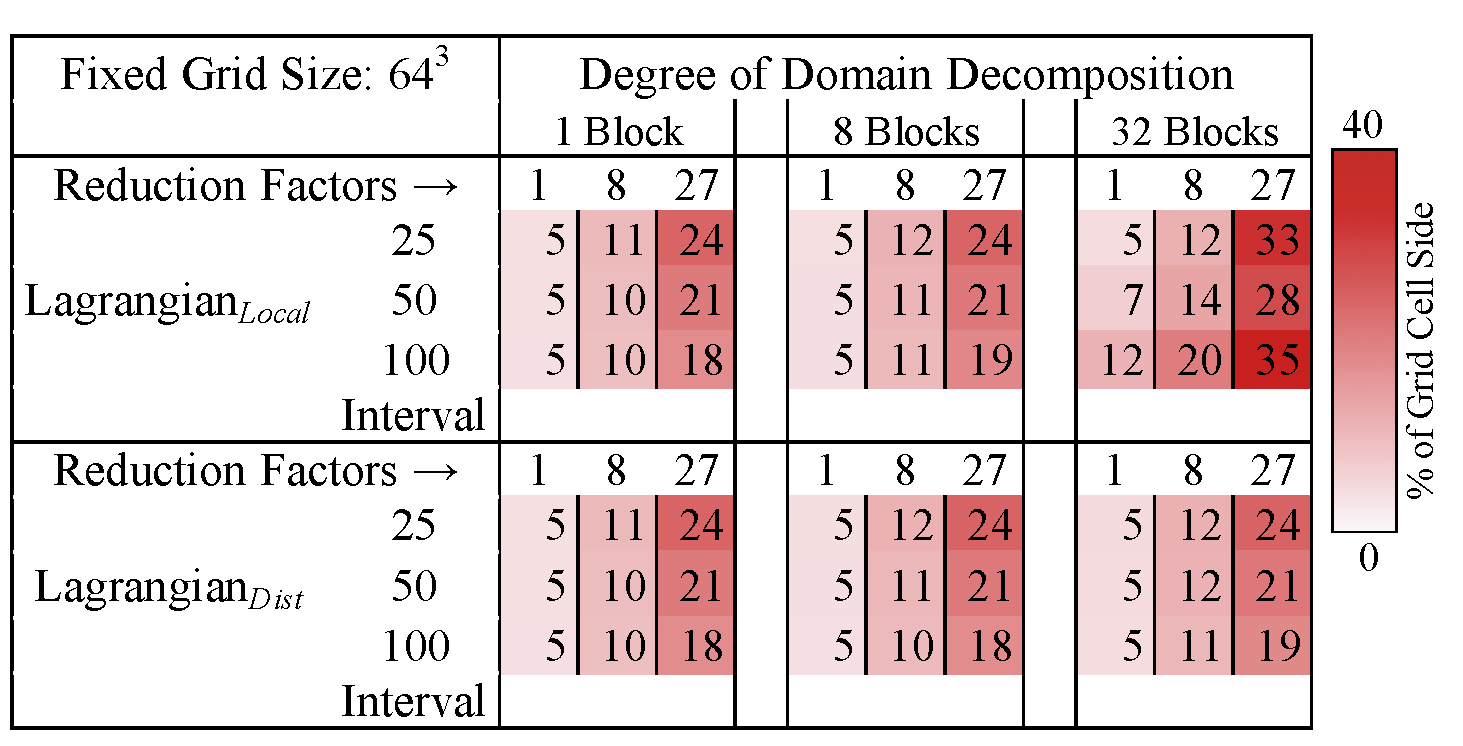
\includegraphics[width=0.95\linewidth]{Images/strongscaling.pdf}
\caption{Average error of new pathlines traced using Lagrangian$_{Dist}$ and Lagrangian$_{Local}$ for varying domain decomposition, storage interval, and data reduction factor. Here, a $64^{3}$ Cloverleaf3D data set defined over 800 cycles is used. Accuracy measurements are compared to the ground truth.} 
\vspace{-5mm}
\label{fig:strongscaling}
\end{figure}

%
Multiphysics HPC simulations typically have millions of grid points per rank and increase grid resolution as the number of ranks increases. 
%
To identify limitations, we evaluated Lagrangian$_{Local}$ in situations where this was not the case, i.e., when the number of processes operating over a fixed grid size increased.
%
%Although multiphysics HPC simulations typically have hundreds of thousands of grid points per data block, we evaluate Lagrangian$_{Local}$ in situations where this is not the case and the number of processes operating over a fixed grid increases .
%

Since the Lagrangian$_{Local}$ strategy was to discard trajectories exiting the rank-specific domain, this approach was susceptible to low resolution data blocks (i.e, sampling would use a small number of particles per rank) and longer storage intervals (i.e., integration times).
%
This experiment measured the error of $1,000$ new pathlines generated for 800 cycles compared to the ground truth. 
%
Further, three parameter options were considered for domain decomposition, storage interval, and data reduction factor. 
%
Figure~\ref{fig:strongscaling} shows the pathline error when interpolating the flow maps generated by Lagrangian$_{Dist}$ and Lagrangian$_{Local}$. 
%
The accuracy of Lagrangian$_{Local}$ remained close to Lagrangian$_{Dist}$ until the domain decomposition is at its highest ($64^{3}$ grid decomposed across 32 ranks).
%
%
Although the overall accuracy of the interpolated pathlines was high (within a single GCS on average for all tests), both techniques lost some accuracy as the storage interval and data reduction factor increased, with Lagrangian$_{Local}$ performing worse under greater domain decomposition.
%
These results highlight the limitations of the Lagrangian$_{Local}$ technique as is.
%
%That said, we discuss approaches that could mitigate these limitations in Section~\ref{sec:discussion}.

%\vspace{-2mm}
\begingroup
\vspace{-2mm}
\begin{table}[!h]
\centering
\caption{Comparison of Lagrangian$_{Local}$ and the traditional approach, i.e., the Eulerian representation with temporal subsampling, for the Cloverleaf3D dataset. The error is the average percentage of grid cell side and is computed for 100,000 pathlines over 600 cycles. The unit for storage is GB.}
\resizebox{\columnwidth}{!}{%
\begin{tabular}{|c||c|c|c|c|}
\hline
Storage & \multicolumn{2}{c|}{Lagrangian$_{Local}$} & \multicolumn{2}{c|}{Eulerian} \\
Interval & Avg \% of GCS & Storage & Avg \% of GCS & Storage \\
\hline
20 & 18.8 & 34 & 115.4 & 267 \\
40 & 25.2 & 17 & 269.0 & 133 \\
60 & 37.5 & 12 & 424.8 & 95 \\
\hline
\end{tabular}
}
\label{clover_eul_table}
\end{table}
\endgroup

\subsubsection{C-II Results} 
Here, we compared Lagrangian$_{Local}$ to using an Eulerian representation with temporal subsampling.
%
Table~\ref{clover_eul_table} shows the results of \textbf{C-II}.
%
We considered three storage intervals: 20, 40, and 60.
%
We used 96 MPI ranks distributed across 16 CNs and a grid size of $586^3$.
%
Lagrangian$_{Local}$ used a data reduction of 1:8, whereas for the Eulerian technique we stored the full spatial resolution.
%
To compare accuracy, we reconstructed 100,000 randomly seeded pathlines for 600 cycles.
%
%
Overall, Lagrangian$_{Local}$ was increasingly accurate (6x to 11x) compared to the Eulerian approach as the interval size increases, but required less data storage.
%
These results aligned with findings in prior works~\cite{agranovsky2014improved, sane2018revisiting} that compared the use of Lagrangian representations to the traditional approach under sparse temporal settings.

%\vspace{-2mm}
\subsection{Phase-II Results Using ABC, Nyx, Jet Data Sets}
This section presents results for three time-varying data sets.
%
We considered a fixed amount of compute resources and varied configuration parameters that impact both execution time and reconstruction accuracy.
%
Figure~\ref{fig:dataset_timings} contains the computation costs for all \textbf{Phase-II} experiments.
\begin{figure}[h]
\centering
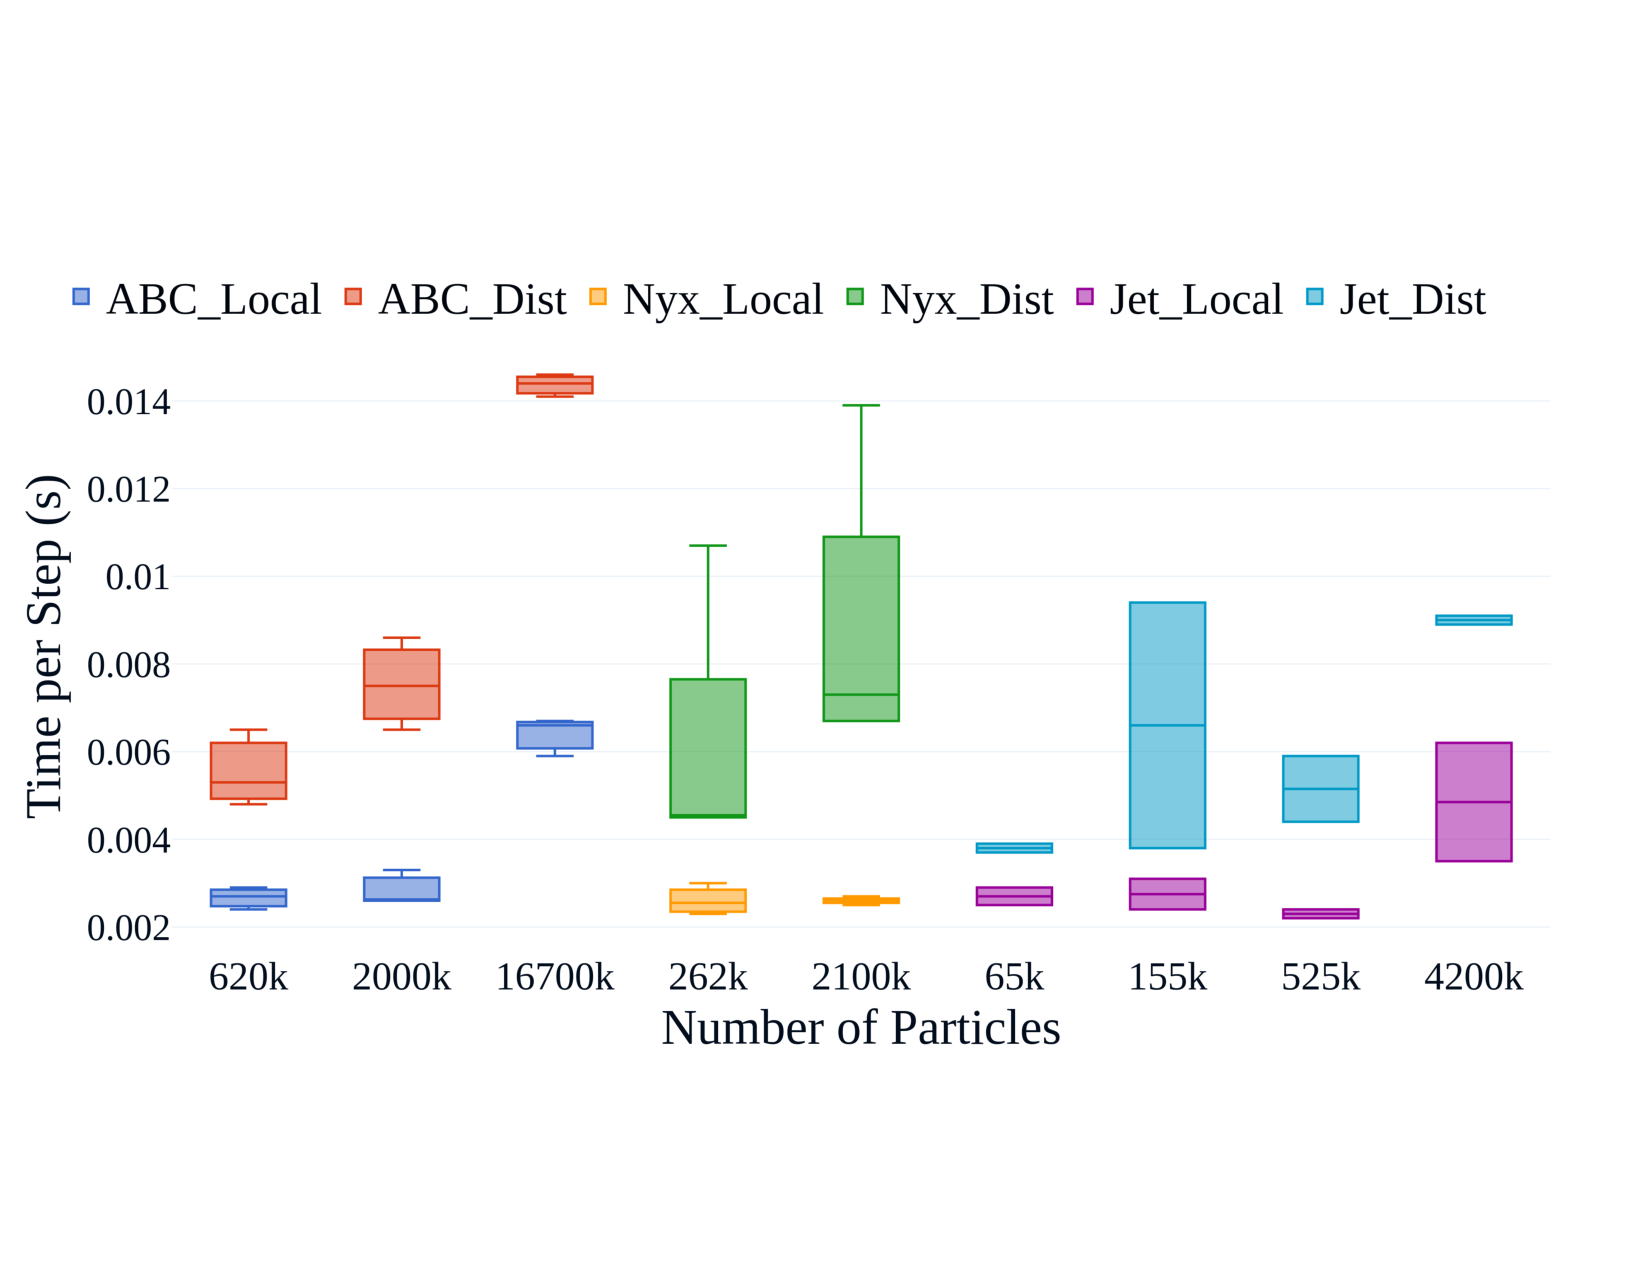
\includegraphics[width=\linewidth, trim={0.45cm 3.5cm 2cm 4.5cm}, clip]{Images/dataset_timings4.pdf}
\caption{Execution time per step of Lagrangian$_{Dist}$ and Lagrangian$_{Local}$ grouped by data set and ordered by the number of particles for \textbf{Phase-II} experiments.}
\label{fig:dataset_timings}
\end{figure}

\label{sec:experiment2}
%\vspace{-2mm}
\subsubsection{ABC Flow}
\label{sec:abc}

Table~\ref{abc_tab} lists all the ABC \textbf{Phase-II} test configurations.
% and Figure~\ref{fig:abc_plot} shows the distribution of trajectory reconstruction error for each test.
%
\begingroup
\begin{table}[h]
\centering
\scalebox{0.9}{
%\resizebox{\columnwidth}{!}{
\begin{tabular}{|c||c|c|c|c|c|c|}
\hline
\textbf{Test} & \textbf{Interval} & \textbf{Reduction} & \textbf{Particles} & \textbf{Stored} & \textbf{Discarded} \\
\hline
T1 & 25 & \multirow{3}{*}{1:1} & \multirow{3}{*}{16700k} & 96.9\% & 3.1\% \\
T2 & 50 & & & 94.3\% & 5.7\%  \\
T3 & 100 & & & 89.7\% & 10.3\% \\
\hline
T4 & 25 & \multirow{3}{*}{1:8} & \multirow{3}{*}{2098k} & 97.7\% & 2.3\% \\
T5 & 50 & & & 95.2\% & 4.8\% \\
T6 & 100 & & & 90.6\% & 9.4\% \\
\hline
T7 & 25 & \multirow{3}{*}{1:27} & \multirow{3}{*}{621k} & 98.6\% & 1.4\% \\
T8 & 50 & & & 95.9\% & 4.1\% \\
T9 & 100 & & & 91.8\% & 8.2\% \\
\hline
\end{tabular}
}
\caption{\fix{Specifications for 9 ABC tests. In most cases, over 90\% of the complete flow map was stored.}}
\vspace{-2mm}
\label{abc_tab}
\end{table}
\endgroup

\begin{figure}[!b]
\vspace{-4mm}
\centering
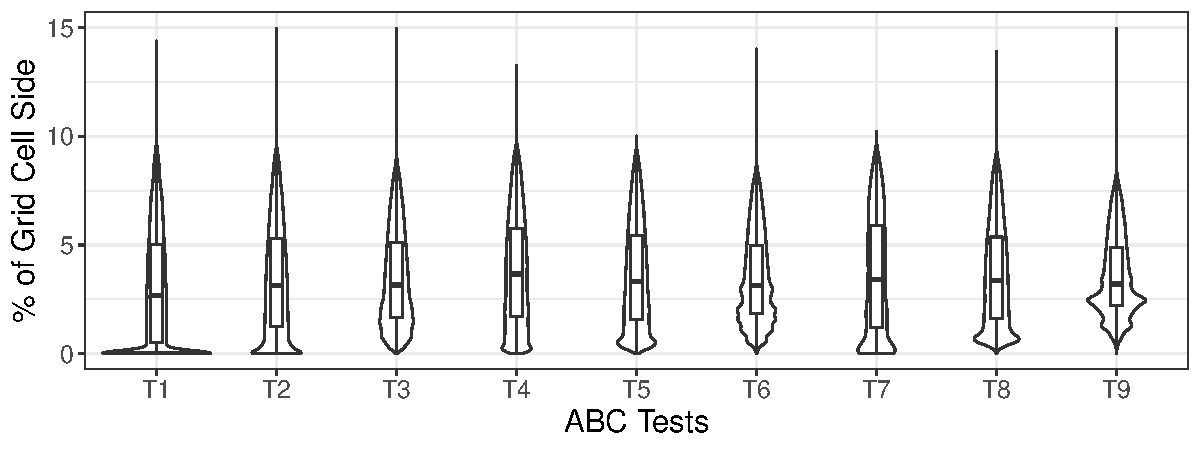
\includegraphics[width=\linewidth]{Images/ABC_Tests.pdf}
\caption{\fix{Violin plots of reconstruction error for the ABC data set tests labeled T1-T9. The plots show the error remained within a consistent range across tests, with only small increases as the data reduction factor and storage interval increase.}}
%\caption{Distribution of reconstruction error for ABC tests.}
\vspace{-2mm}
\label{fig:abc_plot}
\end{figure}


\textbf{Execution Time.} Using 64 MPI ranks across 16 CNs, each with 1 GPU, Lagrangian$_{Local}$ required up to 2.8x less execution time as Lagrangian$_{Dist}$.
%
Figure~\ref{fig:dataset_timings} shows particle advection and communication costs are directly proportional to the particle count.
%
Further, particle advection for up to 2M particles~(32k particles per GPU) was performed in under 0.004 seconds per step for all data sets.
%
\begin{figure}[!ht]
\begin{subfigure}{\linewidth}
\centering
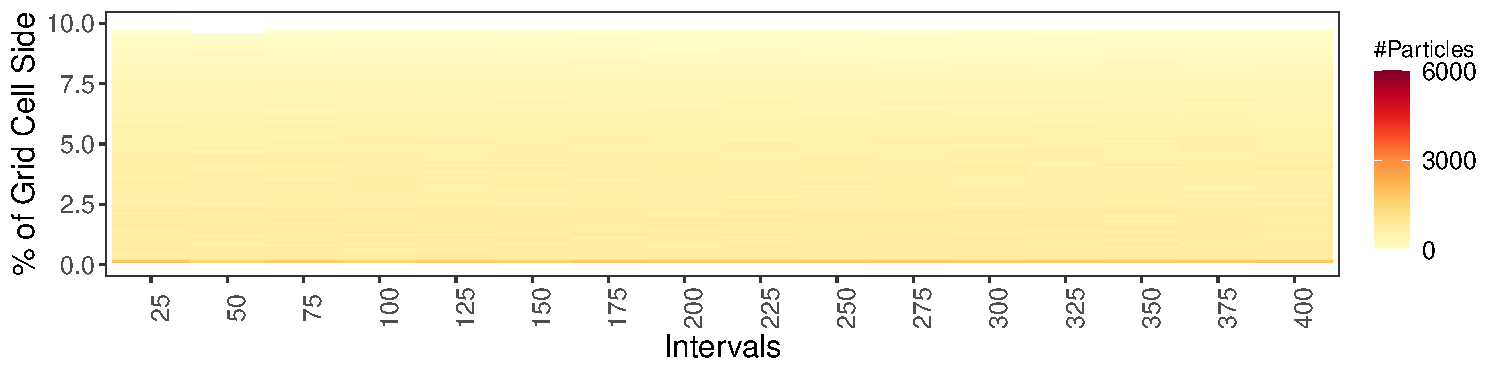
\includegraphics[width=\linewidth]{Images/ABC_Intervals_T4.pdf}
\vspace{-5mm}
\caption{T4, storage interval = 25 cycles}
\label{fig:abc_4}
\end{subfigure}
%\begin{subfigure}{\linewidth}
%\centering
%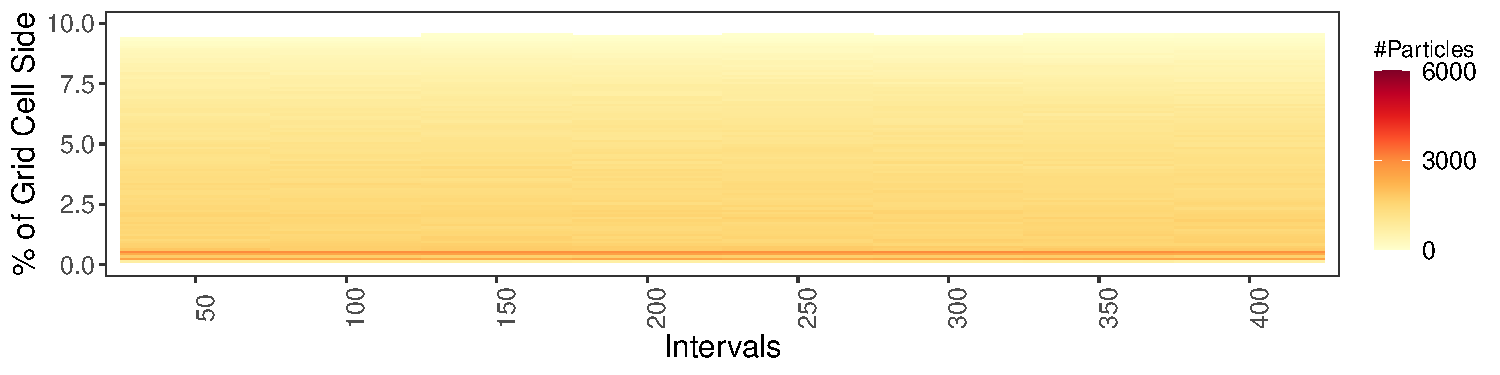
\includegraphics[width=\linewidth]{Images/ABC_Intervals_T5.pdf}
%\caption{T5, storage interval = 50 cycles}
%\label{fig:abc_5}
%\end{subfigure}
\begin{subfigure}{\linewidth}
\centering
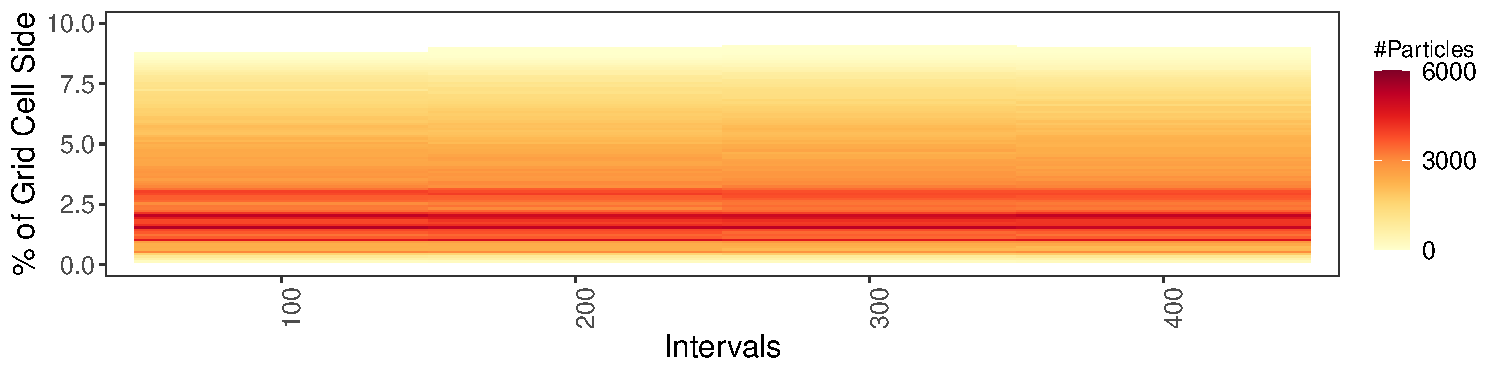
\includegraphics[width=\linewidth]{Images/ABC_Intervals_T6.pdf}
\vspace{-5mm}
\caption{T6, storage interval = 100 cycles}
\label{fig:abc_6}
\end{subfigure}
\caption{\fix{Heatmap of reconstruction error for the ABC data set as a function of interval. These plots show that the majority of reconstructed trajectories are within a grid cell side of the ground truth, despite the larger of number of discarded particles resulting from the larger storage interval~(\ref{fig:abc_6}).}}
%\caption{\fix{For the ABC data set, although increasing the storage interval resulted in a larger number of discarded particles, the majority of reconstructed trajectories are within a grid cell side of the ground truth.}} 
%\caption{ABC data set tests showing impact of variation in storage interval on the distribution of reconstruction error.}
\vspace{-5mm}
\label{fig:abc_map}
\end{figure}


\textbf{Reconstruction Accuracy.} Figure~\ref{fig:abc_plot}'s violin plots indicate the ABC data set shows shifts in reconstruction error distribution when varying the storage intervals and sampling resolution. 
%
Further, the error range for all configurations was similar.
%
Overall, the discarded trajectories from the ABC data set Lagrangian flow map were reconstructed accurately, with trajectories interpolated to the same grid cell as the ground truth.
%
Specifically, for all 9 tests the mean reconstruction error was between 2.5\% and 5\% of GCS from the ground truth.
%

\textbf{Impact of Varying Storage Interval.} Figure~\ref{fig:abc_map} shows heatmaps of the reconstruction error across all intervals for tests T4 and T6.
%
We showed the absolute number of particles reconstructed for each storage interval for a more straightforward comparison between heatmaps.
%
Comparing these heatmaps, the effect of increasing the storage interval was that a larger number of particles were terminated in a single interval and thus reconstruction error increased. 
%
%Further, the reconstruction error distribution matched the corresponding violin plots in Figure~\ref{fig:abc_plot}. 
%
Figure~\ref{abc_ftle} visualizes an FTLE field derived using the T6 Lagrangian$_{Local}$ flow map and annotates a discontinuity in the FTLE field caused by discarded particles.
%Even for longer storage intervals, the error remained small, and the majority discarded trajectories were reconstructed with high accuracy for the ABC data set.

%\vspace{-2mm}
\subsubsection{Nyx Cosmology}
\label{sec:nyx}
Table~\ref{nyx_tab} lists all the Nyx \textbf{Phase-II} test configurations. 
%, Figure~\ref{fig:dataset_timings} contains computation costs, and Figure~\ref{fig:nyx_plot} shows the distribution of trajectory reconstruction error for each test.
%
\begingroup
\begin{table}[!h]
\centering
\scalebox{0.9}{
%\resizebox{\columnwidth}{!}{%
\begin{tabular}{|c||c|c|c|c|c|c|}
\hline
\textbf{Test} & \textbf{Interval} & \textbf{Reduction} & \textbf{Particles} & \textbf{Stored} & \textbf{Discarded} \\
\hline
T1 & 10 & \multirow{4}{*}{1:1} & \multirow{4}{*}{2097k} & 96\% & 4\% \\
T2 & 20 & & & 92.1\% & 7.9\% \\
T3 & 40 & & & 85.7\% & 14.3\%  \\
T4 & 50 & & & 83\% & 17\% \\
\hline
T5 & 10 & \multirow{4}{*}{1:8} & \multirow{4}{*}{262k} & 97.4\% & 2.6\% \\
T6 & 20 & & & 93.7\% & 6.3\% \\
T7 & 40 & & & 88.2\% & 11.8\% \\
T8 & 50 & & & 85.8\% & 14.2\% \\
\hline
\end{tabular}
}
%}
\caption{\fix{Specifications for 8 Nyx tests. We observed the largest number of discarded particles for this data set.}}
\vspace{-2mm}
\label{nyx_tab}
\end{table}
\endgroup


\textbf{Execution Time.} Across our 8 tests using the Nyx data set, Lagrangian$_{Local}$ computed a flow map up to 5.2x faster than the corresponding Lagrangian$_{Dist}$ flow map.
%
Additionally, Figure~\ref{fig:dataset_timings} shows the standard deviation was greater for the Lagrangian$_{Dist}$ tests and was caused by the larger number of particles exchanges between ranks for this data set.
%

\textbf{Reconstruction Accuracy.} As a consequence of a large number of particles being discarded by Lagrangian$_{Local}$, the accuracy of reconstruction was impacted for tests with longer storage intervals.
%
7 of 8 tests showed up to the third quartile reconstructing under 100\% of a GCS. 
%
Comparing tests T3 and T4 (1:1 data reduction factor) to tests T7 and T8 (1:8 data reduction factor), although T3 and T4 discarded a greater percentage of samples, they remained more accurate due to the absolute number of particles used to sample the domain.
%
For shorter storage interval lengths (T1, T2, T5, T6), the reconstruction quality was high for both data reduction factors.
%
Figure~\ref{nyx_ftle} shows an FTLE field derived using the T1 Lagrangian$_{Local}$ flow map. 
%
Lastly, Figure~\ref{fig:nyx_map} shows the distribution of error and temporal pattern of communication during the simulation. 
% of a Nyx configuration.

\begin{figure}[!h]
\centering
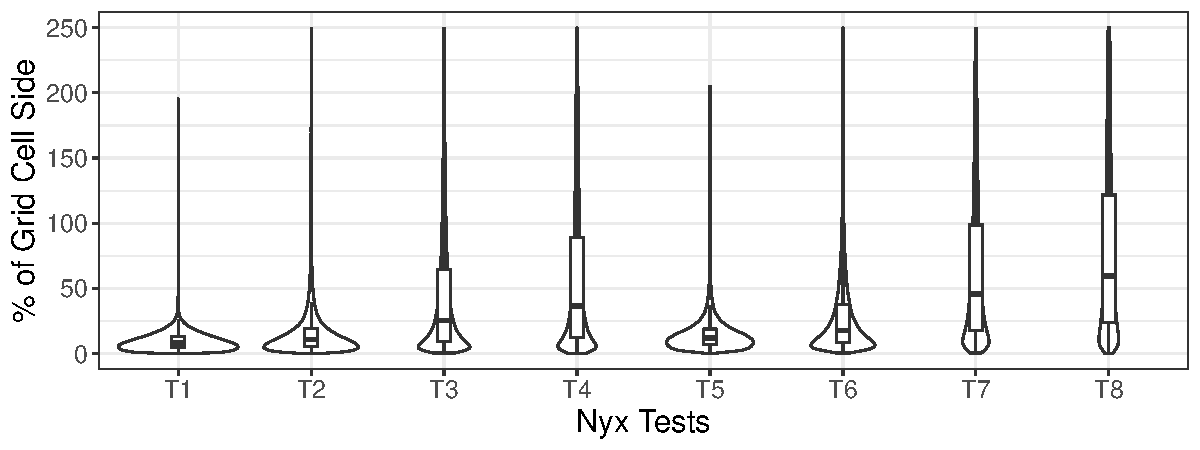
\includegraphics[width=\linewidth]{Images/Nyx_Tests.pdf}
\caption{Distribution of the reconstruction error for Nyx tests.}
\label{fig:nyx_plot}
\end{figure}

\begin{figure}[!h]
\centering
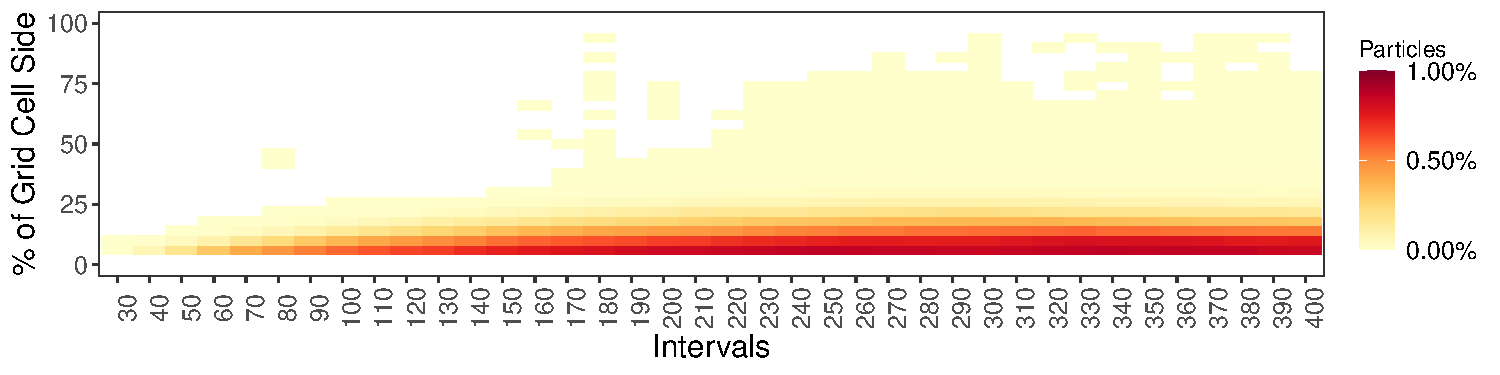
\includegraphics[width=0.95\linewidth]{Images/Nyx_Intervals_T1.pdf}
\caption{The Nyx data set reconstruction error for all the intervals of a single test configuration~(T1).}
\label{fig:nyx_map}
\end{figure}


%\vspace{-2mm}
\subsubsection{Jet Flow}
\label{sec:jet}
Table~\ref{jet_tab} lists all the Jet \textbf{Phase-II} test configurations.
%, Figure~\ref{fig:dataset_timings} contains computation costs, and Figure~\ref{fig:jet_plot} shows the distribution of trajectory reconstruction error for each test.
%
\begingroup
\begin{table}[!b]
\vspace{-2mm}
\centering
\caption{\fix{Specifications for 8 Jet tests. In most cases, under 2\% of particle trajectories are discarded. Accurate reconstruction of these trajectories~(see Figure~\ref{fig:jet_plot}) was dependent on the absolute number of stored particles.}}
\scalebox{0.9}{
%\resizebox{\columnwidth}{!}{%
\begin{tabular}{|c||c|c|c|c|c|c|}
\hline
\textbf{Test} & \textbf{Interval} & \textbf{Reduction} & \textbf{Particles} & \textbf{Stored} & \textbf{Discarded} \\
\hline
T1 & 5 & \multirow{2}{*}{1:1} & \multirow{2}{*}{4194k} & 99.4\% & 0.6\% \\
T2 & 10 & & & 97.9\% & 2.1\% \\
\hline
T3 & 5 & \multirow{2}{*}{1:8} & \multirow{2}{*}{524k} & 99.6\% & 0.4\% \\
T4 & 10 & & & 98.9\% & 1.1\% \\
\hline
T5 & 5 & \multirow{2}{*}{1:27} & \multirow{2}{*}{155k} & 99.7\% & 0.3\% \\
T6 & 10 & & & 99.1\% & 0.9\% \\
\hline
T7 & 5 & \multirow{2}{*}{1:64} & \multirow{2}{*}{65k} & 99.8\% & 0.2\% \\
T8 & 10 & & & 99.3\% & 0.7\% \\
\hline
\end{tabular}
}
\vspace{-2mm}
\label{jet_tab}
\end{table}
\endgroup


\textbf{Execution Time.} For the Jet data set, Lagrangian$_{Local}$ computed a flow map up to 3.9x faster than the corresponding Lagrangian$_{Dist}$ flow map.
%
For this data set, we considered shorter storage intervals, and thus a smaller percentage of particles required particle exchange to continue trajectory integration.
%
However, Figure~\ref{fig:dataset_timings} shows the variability in the cost of communication as it was susceptible to network usage and bandwidth contention.
%
A single outlier Lagrangian$_{Local}$ test showed a higher computation cost. 

\begin{figure}[!b]
\centering
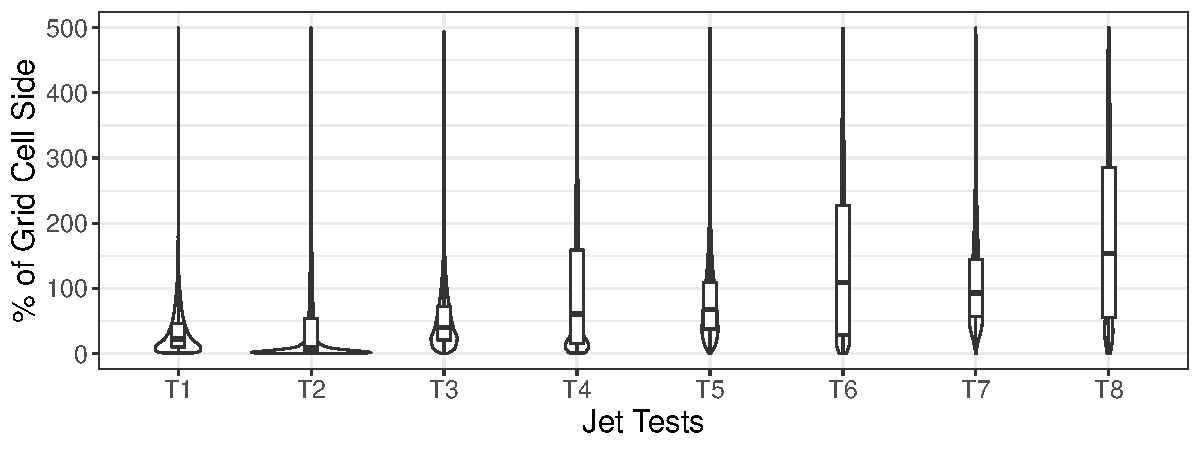
\includegraphics[width=\linewidth]{Images/Jet_Tests.pdf}
\caption{\fix{Violin plots of reconstruction error for the Jet data set tests labeled T1-T8. The plots show that error increased significantly with increased data reduction factor and storage interval. Reconstruction error was low only when no data reduction~(1:1) was used~(T1, T2).}}
%\caption{\fix{As in Figure~\ref{fig:nyx_plot}, reconstruction error for the Jet data set increased significantly with increased data reduction factor and storage interval. We found reconstruction accuracy within a grid cell side for most particles only when no data reduction~(1:1) was used~(T1, T2).}}
%\caption{Distribution of the reconstruction error for Jet tests.}
\vspace{-2mm}
\label{fig:jet_plot}
\end{figure}

\begin{figure}[!b]
\begin{subfigure}{\linewidth}
\centering
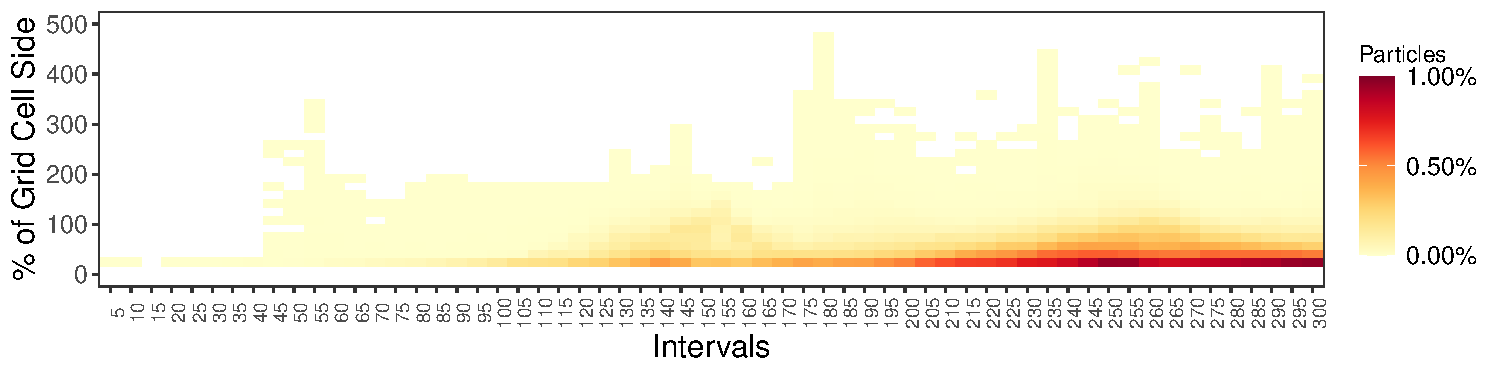
\includegraphics[width=\linewidth]{Images/Jet_Intervals_T1_Percent.pdf}
\caption{T1, 1:1}
\label{fig:jet_1}
\end{subfigure}
\begin{subfigure}{\linewidth}
\centering
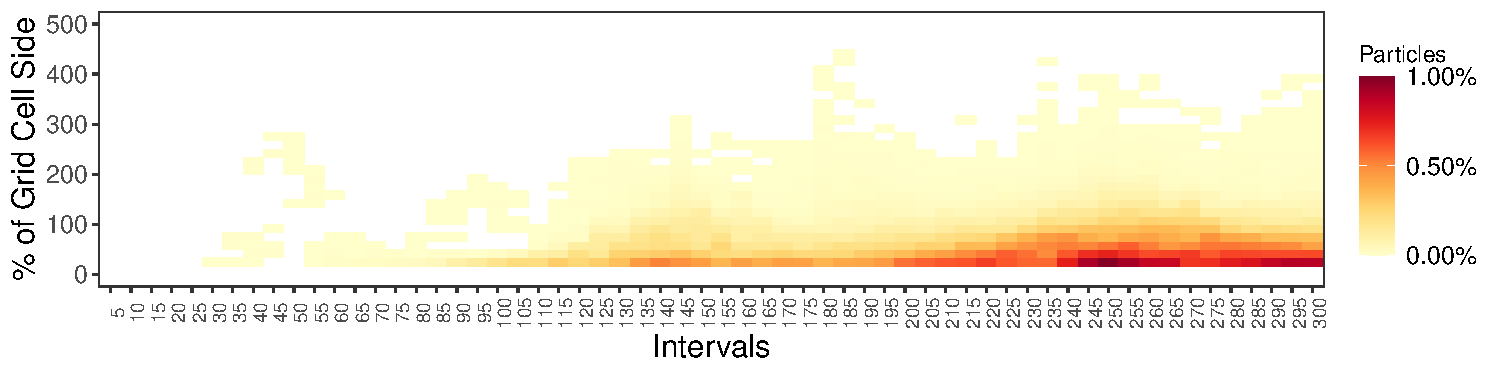
\includegraphics[width=\linewidth]{Images/Jet_Intervals_T3_Percent.pdf}
\caption{T3, 1:8}
\label{fig:jet_3}
\end{subfigure}
\begin{subfigure}{\linewidth}
\centering
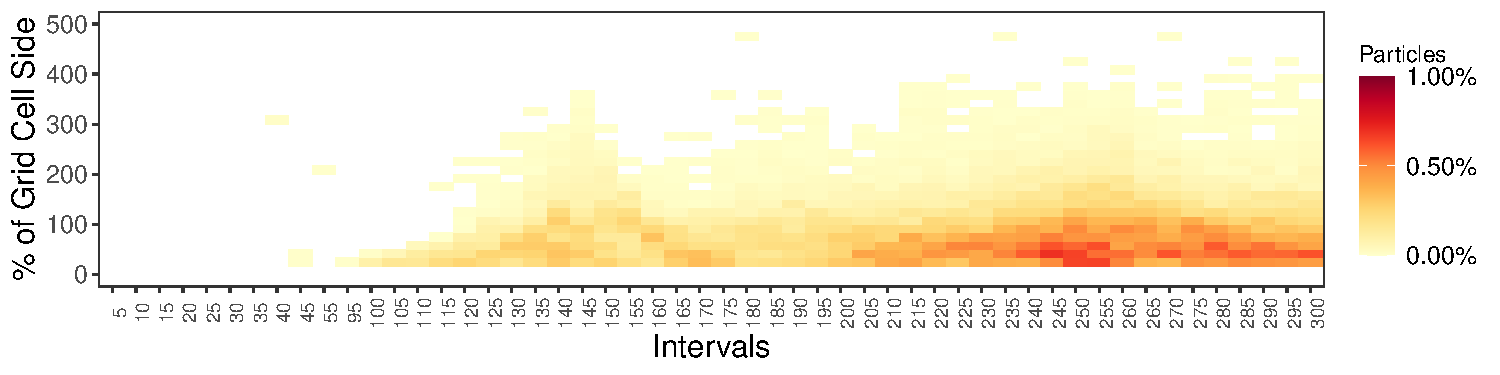
\includegraphics[width=\linewidth]{Images/Jet_Intervals_T5_Percent.pdf}
\caption{T5, 1:27}
\label{fig:jet_5}
\end{subfigure}
\begin{subfigure}{\linewidth}
\centering
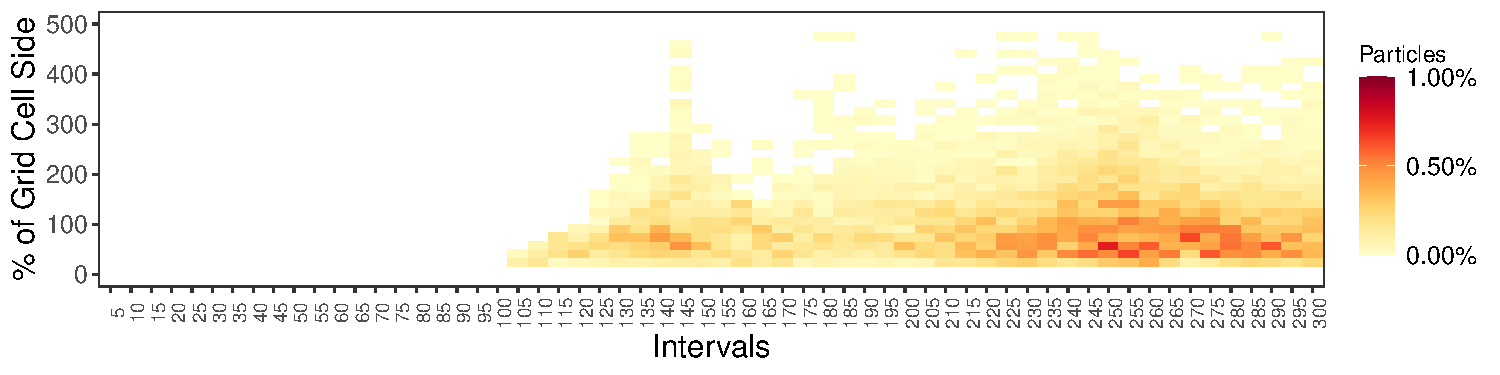
\includegraphics[width=\linewidth]{Images/Jet_Intervals_T7_Percent.pdf}
\caption{T7, 1:64}
\label{fig:jet_7}
\end{subfigure}
\caption{Jet tests showing the impact of variation in the data reduction factor on the distribution of reconstruction error.}
\label{fig:jet_map}
\end{figure}

\textbf{Reconstruction Accuracy.} The Jet data set presented an adversarial case for our proposed optimization of computing local flow maps.
%
The data set contained regions with high velocity magnitude.
%
Across the range of configurations in Figure~\ref{fig:jet_plot}, both the storage interval and the data reduction factor impacted the reconstruction accuracy.
%
6 of 9 tests had a mean reconstruction error under 100\% of GCS. 
%
Further investigation into the distribution of T2 revealed that the longer storage interval and 1:1 sampling resulted in several particles terminating in easy-to-reconstruct areas of the domain at the start of the simulation (most other configurations showed particle termination only after cycle 30).
%
For tests using a storage interval of 10~(T2, T4, T6, T8), the reconstruction accuracy is reduced.
%
%The sparser sampling for other configurations with the same storage interval missed this effect.
%
Figure~\ref{jet_ftle} visualizes an FTLE field derived using the T2 Lagrangian$_{Local}$ flow map and annotates regions of reduced quality reconstruction.
%
However, since the absolute number of particles stored for this test remained high at 97.9\%, most of the FTLE field structure was well reconstructed.
%
%Further, as the number of samples used reduces, the reconstruction of discarded trajectories can be multiple cells away from the ground truth.
%
%For example, T8 using 1:64 data reduction factor and a storage interval of 10, has a mean reconstruction of 150% of GCS.

\textbf{Impact of Varying Data Reduction Factor.} Figure~\ref{fig:jet_map} compares the distribution of reconstruction error as the data reduction factor increases. 
%
Each cell in the heatmap shows a percentage of particles to enable comparison between tests.
%
For test T1 using a 1:1 sampling, reconstruction accuracy was high and a larger percentage of particles were reconstructed with error under 100\% of GCS.
%
As the number of particles used to sample the domain reduced, a higher percentage of particles were reconstructed multiple cells away from the ground truth. 
%
For example, in Figure~\ref{fig:jet_7} test T7 used a 1:64 data reduction factor and there are more red/orange cells with higher error during the later stages of the simulation. 
%
%Based on the distribution of error, the reconstruction accuracy is high when a 1:1 data reduction factor is used, and reduces in accuracy with fewer samples.
%
%Overall, as the number of particles used to sample the domain reduces the mean reconstruction error increases, with tests using a longer storage interval showing higher error.
%
%
%Overall, based on the distribution of reconstruction accuracy, the probability of accurate reconstruction increases with more samples.

